\documentclass[a4paper, 11pt]{article}
\usepackage[utf8]{inputenc}

\usepackage[french]{babel}
\usepackage{graphicx} 
\usepackage{hyperref}
\usepackage{xcolor}
\usepackage{listings}
\usepackage{amsmath} 
\usepackage{amsfonts}
\usepackage{hyperref}
\usepackage{enumitem}
\usepackage[left=2cm, right=2cm, bottom=2cm, top=2cm]{geometry}
\newcommand{\HRule}{\rule{\linewidth}{0.5mm}}


\begin{document}
\begin{titlepage}


\begin{center}

\includegraphics[scale = 0.35]{logo.jpg}\\
\vspace{1cm}
\textsc{\huge université de Liège}\\[1.2cm]
\HRule \\[1cm]
\textsc{\LARGE Eléments de statistiques}\\[1cm]
{\Huge \bfseries Devoir}\\[1.4cm] 
\HRule \\[1cm]
    
\end{center}

\begin{minipage}{0.4\textwidth}
      \begin{flushleft} \large
        \emph{Auteurs : } \\
        Louis \textsc{Hogge} S192814\\
        Hugo \textsc{Jacobs} S193340\\
     
      \end{flushleft}
\end{minipage}
\begin{minipage}{0.45\textwidth}
      \begin{flushright} \large
        \emph{Professeur : } P. \textsc{Sacré}\\
        \emph{Année : } 2021-2022
      \end{flushright}
\end{minipage}
\end{titlepage}

\section{Analyse descriptive}
\begin{enumerate}[label=(\alph*)] 
    \item  Dans le tableau ci-dessous, nous avons extrait les données pour 4 pays.\\
    \\
    \begin{tabular}{|p{4.5cm}||p{3cm}|p{3cm}|p{3cm}|}
    \hline 
       \textbf{Pays}  &  \textbf{PIB\_habitant} & \textbf{CO2\_habitant} & \textbf{Top10} \\
       \hline \hline
        \textit{Etats-Unis} & 47757,5109 & 17,0617465973 & 0,4546\\
       \hline
       \textit{Belgique} & 39506.041 & 15.2828989029 & 0,3289 \\
         \hline
         \textit{Chine} & 15417.9174 & 6.53579044342 & 0.4166 \\
         \hline
         \textit{Togo} & 1234.2999 & 0.998398005962 & 0.4798 \\
         \hline
    \end{tabular}\\\\
    
    Une analyse de ce tableau permet, grâce au choix judicieux des pays, de mettre en lumière les différents ordres de grandeur de chaque variable.
    \\
    \\
    Premèrement, en comparant les valeurs du PIB/habitant des Etats-Unis et du Togo, on prend conscience de l’amplitude de cette variable, la valeur des Etats-Unis prenant le rôle de maximum et celle du Togo celui de minimum. On peut ensuite se laisser surprendre par la valeur du PIB/habitant de la Chine qui est une des plus grosse puissance mondiale. Cependant, en prenant en compte l’importante population du pays on peut aisément comprendre le résultat. Il s'agit du schéma inverse pour la Belgique, un si grand PIB/habitant pour un si petit pays peut étonner, mais en se rappelant que le pays ne comporte qu’un peut plus de 11 millions d’habitants, le résultat semble plausible.
    \\
    \\
    Pour continuer, observons l’empreinte CO2 /habitant, exprimée en tCO2/an. Sans surprise, les résultats sont en corrélations avec les valeurs de PIB/habitant associées à chaque pays, les Etats-Unis jouant le rôle de maximum, le Togo celui de minimum, la Chine et la Belgique expliquant leurs valeurs par leurs nombres d’habitants.
    \\
    \\
    Finalement, examinons le pourcentage de revenu national détenu par les 10$\%$ des habitants les plus aisés de chaque pays. Diverses constations peuvent être faites :
    \begin{itemize}[leftmargin=2cm]
    \item Le Togo, étant le pays le plus pauvre des 4, est, également, celui dans lequel les inégalités sont les plus grandes. 
    \item La Belgique, réputée pour son système social élaboré, est le pays dans lequel les disparités sont les plus faibles.
    \item Les Etats-Unis, régime ultra-libéral, voit logiquement son pourcentage être important.
    \item La Chine, bien qu’officiellement un régime communiste, possède un pourcentage presque aussi élevé que celui des Etats-Unis.  
    \end{itemize}

    \item
    \begin{enumerate}[label=\roman*.]
        \item Les moyennes et les écarts-types des différentes variables sont représentées dans le tableau suivant :\\\\ 
        \begin{tabular}{|p{4cm}||p{4cm}|p{4cm}|}
        \hline
             & \textbf{Moyenne arithmétique} & \textbf{Ecart-Type}\\
             \hline \hline
              \textit{PIB\_habitant} &  19807.011615333326 & 28416.71562511812\\
              \hline
              \textit{CO2\_habitant} & 5.431475711091641 & 5.806706359814826\\
              \hline
              \textit{Top10} & 0.44989466666666666 & 0.09089117453828259\\
              \hline
        \end{tabular}\\
        \item Dans le tableau ci-dessous sont reprises les valeurs des médianes et des quartiles pour les différentes variables: \\\\\
        \begin{tabular}{|p{2.5cm}||p{3cm}|p{3cm}|p{3cm}|}
        \hline
             &  \textbf{Médiane}& \textbf{Premier quartile} &  \textbf{Troisième quartile}\\
             \hline \hline
             \textit{PIB\_habitant} &  12417.8713 &   3944.557225 & 27972.663875\\
             \hline
             \textit{CO2\_habitant}&  3.570141673084997 & 0.928513 & 8.122242
              \\
             \hline
             \textit{Top10}&  0.4547 &   0.378400 &   0.494375 \\
             \hline
        \end{tabular}\\\\
        Les figures suivantes sont des boites à moustaches. Elles illustrent les valeurs obtenues ci-dessus : 
        \begin{itemize}[leftmargin=2cm]
        \item La barre du milieu représente la médiane.
        \item Les extrémités de la boite représentent les premier et troisième quartiles.
        \item Les extrémités des moustaches représentent les valeurs minimale et maximale en dehors de données aberrantes.
        \item Les points représentent les données aberrantes. (il existe donc des données aberrantes)
        \end{itemize}
        En comparant les 3 graphiques on constate que la majorité des valeurs de la variable $Top10$ ainsi que sa médiane se trouvent à mi-distance entre le maximum et le minimum alors que, concernant les variables $PIB\_habitant$ et $CO2\_habitant$, les majorités et les médianes se trouvent bien plus proche du minimum que du maximum. De plus, pour ces mêmes 2 variables, on remarque plusieurs données aberrantes du côté du maximum.
        \\
        \\
        On peut analyser ces observations de la manière suivante : 
        \begin{itemize}[leftmargin=2cm]
        \item Peu de pays possèdent les richesses du monde et polluent la Terre, il existe un déséquilibre inter-pays.
        \item Les disparités de richesses intra-pays sont globalement équilibrées.
        \end{itemize}
        \begin{figure}[h!]
            \centering
            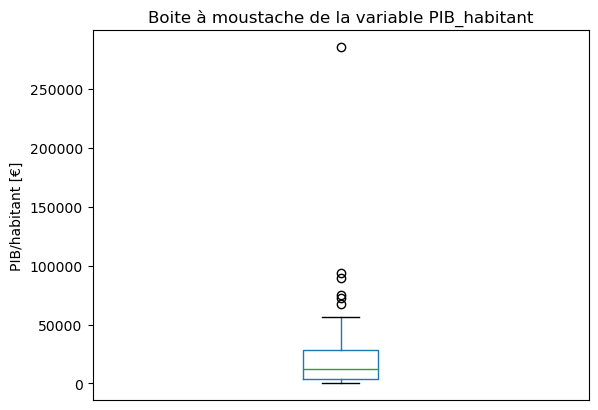
\includegraphics[scale=0.45]{boxplot3.png}
            \caption{}
            \label{fig:my_l}
            \end{figure}
            \begin{figure}[h]
            \begin{minipage}[b]{0.6\linewidth}
                \centering 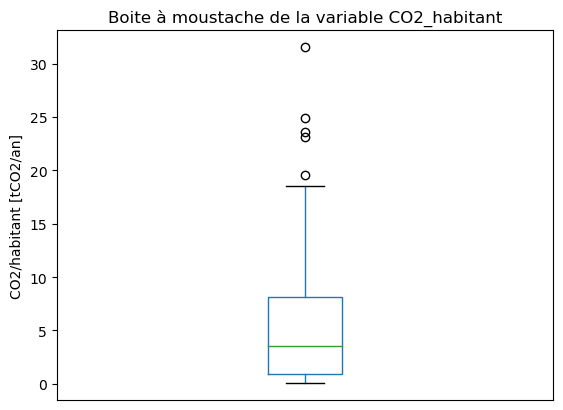
\includegraphics[scale=0.45]{boxplot2.png}
                \caption{}
            \end{minipage}\hfill
            \begin{minipage}[b]{0.4\linewidth}  
                \centering 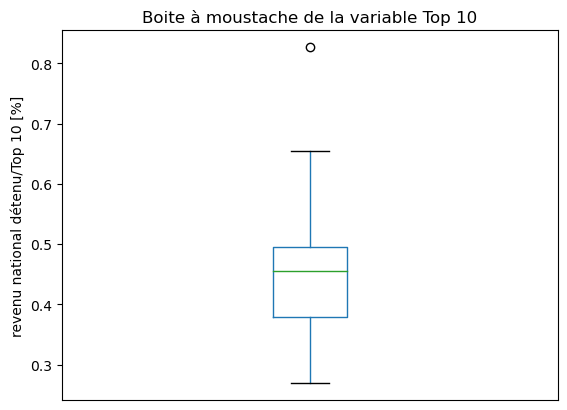
\includegraphics[scale=0.45]{boxplot1.png}
                \caption{}
            \end{minipage}
            \end{figure}
        
        \newpage
        \item Concernant les graphiques de la variable $PIB\_habitant$ et ceux de la variable $Top10$, on peut facilement réaliser les mêmes observations qu'au point précédent (ii.), la majorité et les données aberrantes étant claires.
        \\
        \\
        Grâce aux graphiques relatif à la variable $CO2\_habitant$ on remarque plus aisément la répartition des émissions de CO2/habitant entre pays. On découvre qu'un grand nombre de pays produit très peu de CO2/habitant et que le reste en produit graduellement de plus en plus. Cela représente bien les disparités mondiales en matière d'industrialisation des pays.
    \begin{figure}[h!]
    \begin{minipage}{.5\textwidth}
        \centering
        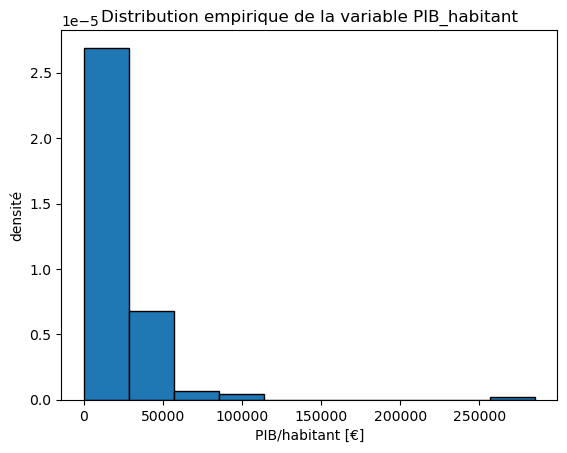
\includegraphics[width=6.5cm]{hist3.png}
        \caption{}
        \label{Débit_frottement}
    \end{minipage}
    \hspace{0.55cm}
    \begin{minipage}{.5\textwidth}
        \centering
        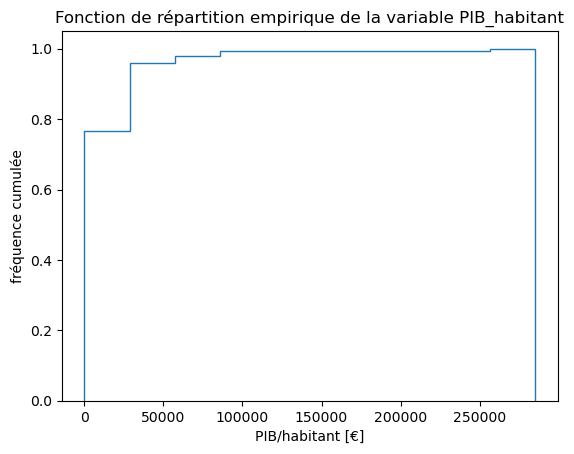
\includegraphics[width=6.5cm]{cdf3.png}
        \caption{}
        \label{Pression_frottement}
    \end{minipage}
\end{figure}
\begin{figure}[h!]
    \begin{minipage}{.5\textwidth}
        \centering
        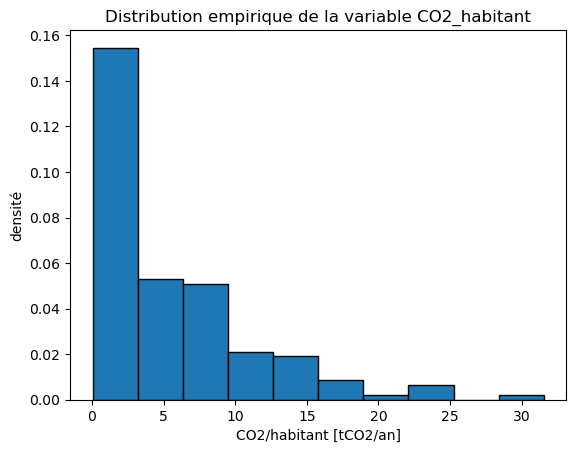
\includegraphics[width=6.5cm]{hist2.png}
        \caption{}
        \label{Débit_frottement}
    \end{minipage}
    \hspace{0.55cm}
    \begin{minipage}{.5\textwidth}
        \centering
        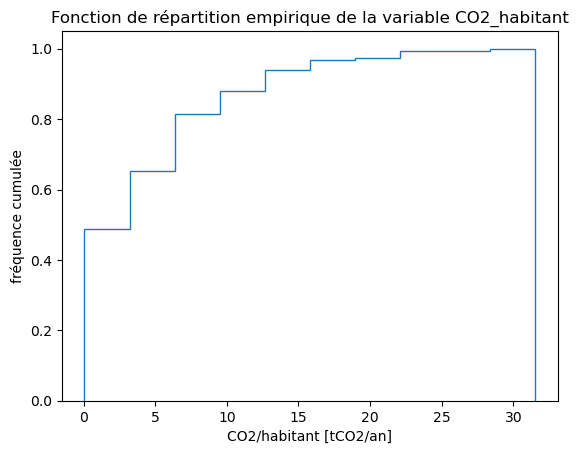
\includegraphics[width=6.5cm]{cdf2.png}
        \caption{}
        \label{Pression_frottement}
    \end{minipage}
\end{figure}
\begin{figure}[h!]
    \begin{minipage}{.5\textwidth}
        \centering
        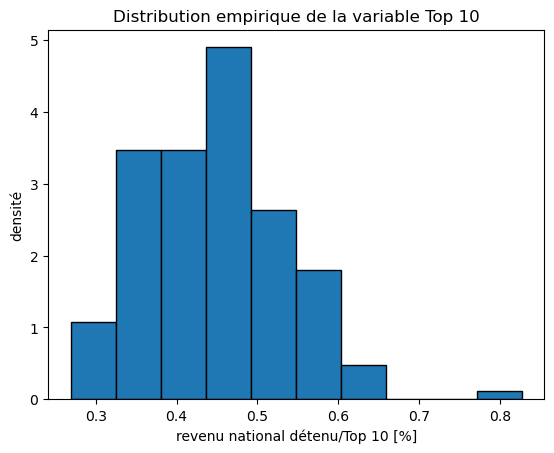
\includegraphics[width=6.5cm]{hist1.png}
        \caption{}
        \label{Débit_frottement}
    \end{minipage}
    \hspace{0.55cm}
    \begin{minipage}{.5\textwidth}
        \centering
        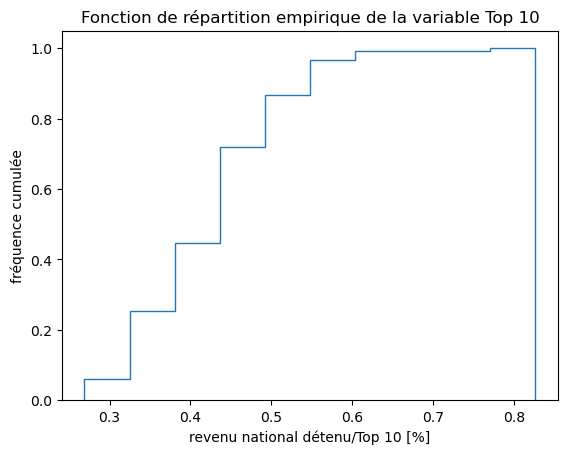
\includegraphics[width=6.5cm]{cdf1.png}
        \caption{}
        \label{Pression_frottement}
    \end{minipage}
\end{figure}
    \end{enumerate}
    \newpage
    \item Pour commencer, on remarque aisément, aussi bien graphiquement que numériquement (tableau point 1(a)) une forte relation linéaire entre les variables $PIB\_habitant$ et $CO2\_habitant$ : plus le PIB/habitant d'un pays augmente plus le CO2/habitant du même pays augmente.
    \\
    \\
    Ensuite, on constate dans un premier temps que plus la variable pourcentage du top 10 d'un pays augmente plus le CO2/habitant à tendance à diminuer, selon relation relativement linéaire. Cependant, la relation (qui n'est déjà pas forte) semble par la suite perdre en force.
    \\
    \\
    Finalement, on observe d'abord que plus la variable pourcentage du Top10 d'un pays augmente plus le PIB/habitant diminue, selon une relation linéaire, et puis que les variables perdent fortement leur relation.
    
    \begin{figure}[h!]
        \centering
        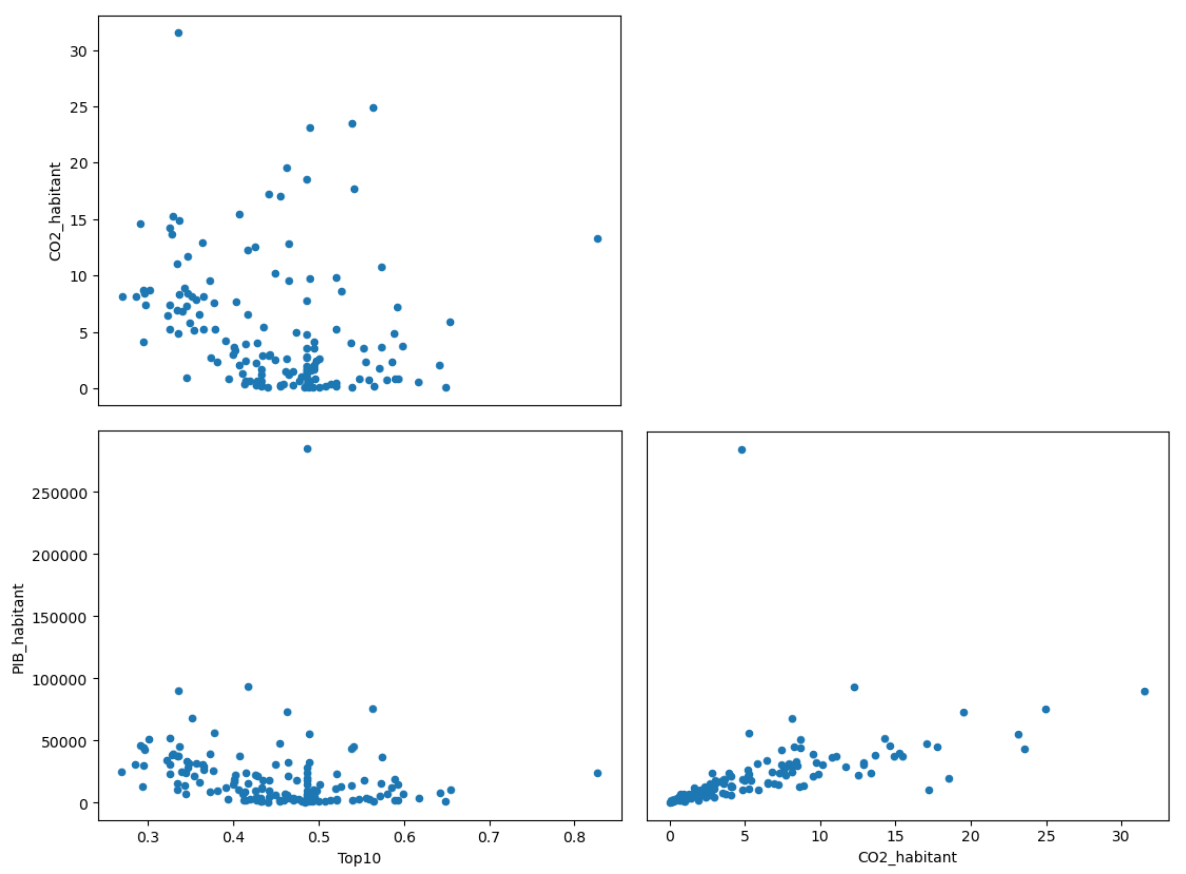
\includegraphics[scale=0.4]{matrix.png}
        \caption{Nuages de points mettant en exergue les relations entre couples de variables}
        \label{fig:my_label}
    \end{figure}
\end{enumerate}

\newpage
\section{Estimation ponctuelle}
\begin{enumerate}[label=(\alph*)]
    \item On souhaite démontrer mathématiquement les formules des estimateurs $\^a_{MOM}$ et $\^b_{MOM}$. Ceux-ci sont des estimateurs des paramètres du modèle statistique de la variable $Top_{10}$. Ce dernier suit une distribution $Beta(a,b)$. Les formules doivent être déterminées par la méthode des moments. Soit $Y$ la variable aléatoire correspondant à la valeur du $Top_{10}$. On sait alors que $Y \sim Beta(a,b)$ et que, par conséquent, si $s$ est l'écart type de l'échantillon étudié:
    $$E(Y)=\frac{a}{a+b} ~et~s^2=\frac{ab}{(a+b)^2(a+b+1)}$$ 
    Pour un échantillon de $Y$ nous avons :
    $$E(Y)=\overline{Y}=\frac{1}{n}\sum^n_{i=1} Y_i~\Longleftrightarrow~\frac{a}{a+b}=\overline{Y}$$
    De cette équation nous déduisons :
    $$b=\frac{a(1-\overline{Y})}{\overline{Y}}$$
    En injectant la valeur de $b$ dans l'expression de l'écart-type et en simplifiant au maximum nous obtenons :
    $$s^2=\frac{\overline{Y}^2(1-\overline{Y})}{a+\overline{Y}}$$
    En isolant $a$ nous trouvons:
    $$\^a_{MOM}=\overline{Y}\left[\frac{\overline{Y}(1-\overline{Y})}{s^2}-1\right]$$
    Par conséquent:
    $$\^b_{MOM}=\frac{(\overline{Y}-\overline{Y}^2+s^2)(1-\overline{Y})}{s^2}$$
    Nous avons désormais les formules des estimateurs des paramètres du modèle statistique.
    \item Maintenant que nous avons ces formules, nous pouvons calculer les valeurs de ces paramètres pour un échantillon composé du $Top10$ de 50 pays pris au hasard parmi notre population. Pour cela, nous devons calculer la moyenne et  l'écart-type de cet échantillon. Nous obtenons ainsi:
    $$\^a_{MOM}=19,60724~et~\^b_{MOM}25,61333$$
    \item La seconde méthode pour déterminer les estimateurs des paramètres est de déterminer les estimateurs du maximum de vraisemblance. Cependant, il n'existe pas de formule analytique pour la maximum de vraisemblance, mais on peut le déterminer numériquement en maximisant la fonction de log-vraisemblance suivante:
    $$ log L(a,b;\textbf{y})= (a-1)\sum_{i=1}^n log(y_i) +  (b-1)\sum_{i=1}^n log(1-y_i) -n log\left(\frac{\Gamma(a) \Gamma(b)}{\Gamma (a+b)}\right)$$
    En effet, la fonction de vraisemblance d'une distribution $Beta(a,b)$ est donnée par :
    $$L(a,b,\textbf{y})=f_{\textbf{Y}}(a,b;\textbf{y})=\prod_{i=1}^n f_Y(a,b;y_i)$$
    où $f_Y(a,b;y_i)$ est la PDF d'une distribution $Beta(a,b)$, et vaut donc $f_Y(a,b;y_i)=\frac{\Gamma(a+b)}{\Gamma(a) \Gamma(b)} y_i^{(a-1)} (1-y_i)^{(b-1)}$.
    On obtient ainsi la forme de la fonction de vraisemblance :
    $$L(a,b;\textbf{y})=\prod^n_{i=1} \frac{\Gamma(a+b)}{\Gamma(a) \Gamma(b)} y_i^{(a-1)} (1-y_i)^{(b-1)}$$
    Désormais, en prenant le logarithme de cette expression, nous obtenons:
    $$log L(a,b;\textbf{y})=log\left(\frac{\Gamma(a+b)}{\Gamma(a) \Gamma(b)} y_i^{(a-1)} (1-y_i)^{(b-1)}\right)$$
    $$\Longleftrightarrow log L(a,b;\textbf{y})=(a-1)log(y_i)+(b-1) log(1-y_i)+\underbrace{log\left(\frac{\Gamma(a+b)}{\Gamma(a) \Gamma(b)}\right)^n}_{-nlog\left(\frac{\Gamma(a) \Gamma(b)}{\Gamma (a+b)}\right)}$$
    Cela prouve que la formulation mathématique de la log-vraisemblance d'une distribution $Beta(a,b)$ est bel et bien correcte.
    \item Grâce à cette expression de la log-vraisemblance, il est possible de déterminer les valeurs des estimateurs des paramètres $a$ et $b$ déterminés par la méthode du maximum de vraisemblance sur le même échantillon qu'au point 2(b), $\^a_{MLE}$ et $\^b_{MLE}$. Et ce à l'aide des fonctions \textbf{beta\_loglikelihood} et \textbf{scipy.optimize.minimize}. Après calcul, nous obtenons:
    $$\^a_{MLE}=20,17676~et~\^b_{MLE}=25,20644$$
    \item Regardons si les estimateurs que nous venons de calculer sont une bonne estimation des vrais paramètres de la distribution $Beta(a,b)$. Pour ce faire, nous superposons, pour chacune des deux méthodes, les histogrammes de notre échantillon de 50 pays et les distributions $Beta(\^a,\^b)$ et nous vérifions si celles-ci présentent des formes similaires. L'histogramme de notre population est, par soucis de clarté, normé. Les figures suivantes présentent ces résultats :
        \begin{figure}[h!]
    \begin{minipage}{.5\textwidth}
        \centering
        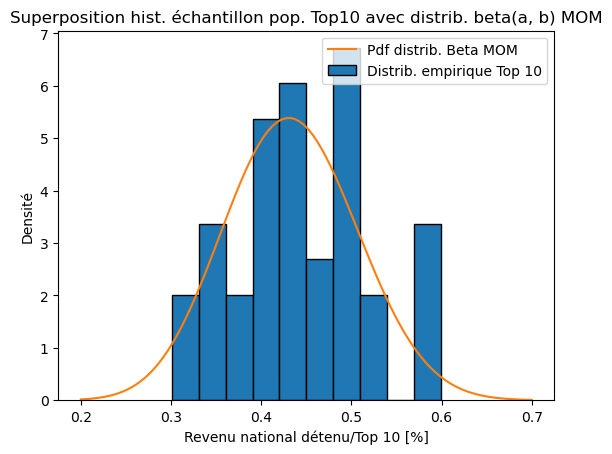
\includegraphics[width=8cm]{superpo_MOM.png}
        \caption{}
        \label{Débit_frottement}
    \end{minipage}
    \hspace{0.55cm}
    \begin{minipage}{.5\textwidth}
        \centering
        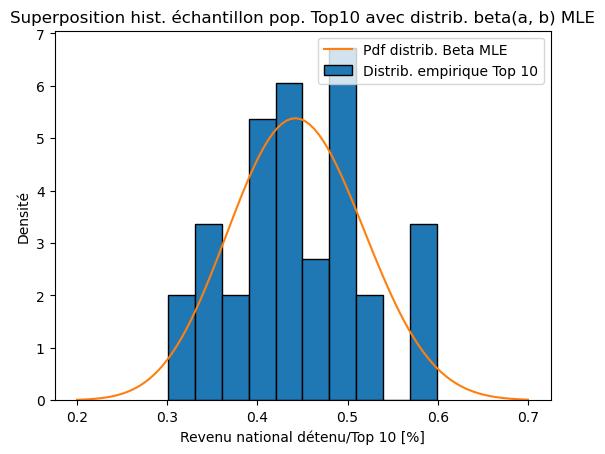
\includegraphics[width=8cm]{superpo_MLE.png}
        \caption{}
        \label{Pression_frottement}
    \end{minipage}
\end{figure}\\\\
On peut conclure, en regardant ces deux graphiques, que les estimateurs des paramètres que nous avons calculés sont des estimations relativement bonnes. En effet, la pdf de la distribution $Beta$ calculée avec nos estimateurs et l'histogramme de notre population présentent des formes similaires. En observant plus précisément, il semblerait que la pdf de la distribution $Beta$ où les paramètres sont calculés avec la méthode des moments, épouse sensiblement mieux l'histogramme de notre population.

    \item Maintenant, supposons que nous connaissons les vrais valeurs des paramètres $a$ et $b$ de la distribution $Beta(a,b)$. Ceux-ci valent $a=13,35$ et $b=16,31$. Nous pouvons ainsi nous intéresser à la qualité de nos estimateurs. Pour ce faire, nous calculons ceux-ci via la méthode des moments, $\^a_{MOM}$ et $\^b_{MOM}$, pour 500 échantillons aléatoires de 50 pays. Nous obtenons dès lors deux populations, une pour chacun des estimateurs, qui vont nous permettent de calculer les biais, variances et erreurs quadratiques moyenne. Les résultats sont repris dans le tableau suivant :
    \begin{center}
    \begin{tabular}{|p{1.5cm}||p{3.5cm}|p{3.5cm}|p{3.5cm}|}
    \hline
         & \textbf{Biais} & \textbf{Variance} & \textbf{Erreur quadratique moyenne} \\
         \hline \hline
      \^a_{MOM} & 0,13180 & 6,88189 & 6,89926  \\
      \hline
      \^b_{MOM} & 1,32163 & 11,23885 & 12,98556 
      \\ 
      \hline
    \end{tabular}
    \end{center}
    \item Nous effectuons ensuite exactement la même opération qu'au point (f), mais pour des estimateurs calculés à l'aide du maximum de vraisemblance. Les résultats sont repris dans le tableau suivant:
       \begin{center}
    \begin{tabular}{|p{1.5cm}||p{3.5cm}|p{3.5cm}|p{3.5cm}|}
    \hline
         & \textbf{Biais} & \textbf{Variance} & \textbf{Erreur quadratique moyenne} \\
         \hline \hline
      \^a_{MLE}   & 0,38025 & 7,85826 & 8,00285 \\
      \hline
      \^b_{MLE} & 0,50513 & 13,05421 & 13,30937 \\
      \hline
    \end{tabular}
    \end{center}
    \item En observant les résultats obtenus via les deux méthodes ci-dessus, nous pouvons dire plusieurs choses:
    \begin{itemize}
        \item Le biais d'un estimateur est une estimation de la précision de la moyenne d'un estimateur. La formule du biais étant donnée ici par :
        $$biais(\hat{a})= \left(\frac{1}{500}\sum^{500}_{i=1} \hat{a}_i \right)-a$$
        Donc, plus le biais est faible, plus la moyenne des 500 estimateurs est proche de la valeur du paramètre. Dans les tableaux ci-dessus, le biais de $\hat{a}$ est plus précis selon la méthode des moments, alors que le biais de $\hat{b}$ est plus faible selon la méthode du maximum de vraisemblance. On ne peut donc déterminer la meilleur méthode grâce aux biais des estimateurs.
        \item La variance des estimateurs est plus faible lorsqu'ils sont calculés à l'aide de la méthode des moments. Ceux-ci varient donc, avec cette méthode, moins autour de leur moyenne. 
        \item Les erreurs quadratiques moyennes des estimateurs, sont plus faibles lorsque les estimateurs sont calculées à l'aide de la méthode des moments. L'erreur quadratique est ici donnée par:
        $$MSE(\hat{a})=\frac{1}{500}\sum^{500}_{i=1} (\hat{a}_i-a)^2$$
        %$$biais(\hat{a})= \left(\frac{1}{500}\sum^{500}_{i=1} \hat{a}_i \right)-a$$
        Cette dernière fournit une véritable estimation de la précision de l'estimateur. Par conséquent, on peut estimer que la méthode des moments fournit des estimateurs plus précis.
    \end{itemize}
    Après cette analyse, nous pouvons conclure que la méthode des moments donne les meilleurs estimateurs. En effet, ceux-ci sont les plus précis, et fluctuent moins autour de leur moyenne, ils sont donc plus fiables.
    \item \textbf{BONUS}\\
    Nous avons réalisé la même démarche qu'au point (f) et (g) en tirant différentes tailles d'échantillons. Les résultats sont repris dans les tableaux ci-dessous.
    \begin{center}
    \begin{tabular}{|p{1.5cm}||p{3.5cm}|p{3.5cm}|p{3.5cm}|}
    \hline
        \textit{20 pays} & \textbf{Biais} & \textbf{Variance} & \textbf{Erreur quadratique moyenne} \\
         \hline \hline
      \^a_{MOM} & 1,51807 & 29,65859 & 31,96313  \\
      \hline
      \^b_{MOM} & 3,08386 & 48,41319 & 57,92338 \\
      \hline
      \^a_{MLE}   & 2,34242 & 33,11872 & 38,60564 \\
      \hline
      \^b_{MLE} & 2,99295 & 54,39191 & 63,34964 \\
      \hline
    \end{tabular}
    \end{center}
    
    \begin{center}
    \begin{tabular}{|p{1.5cm}||p{3.5cm}|p{3.5cm}|p{3.5cm}|}
    \hline
        \textit{40 pays} & \textbf{Biais} & \textbf{Variance} & \textbf{Erreur quadratique moyenne} \\
         \hline \hline
      \^a_{MOM} & 0,41401 & 10,40977 & 10,58117  \\
      \hline
      \^b_{MOM} & 1,65222 & 16,60645 & 19,33630 \\
      \hline
      \^a_{MLE}   & 0,72289 & 11,68797 & 12,21054 \\
      \hline
      \^b_{MLE} & 0,91132 & 18,99630 & 19,82680 \\
      \hline
    \end{tabular}
    \end{center}
    
    \begin{center}
    \begin{tabular}{|p{1.5cm}||p{3.5cm}|p{3.5cm}|p{3.5cm}|}
    \hline
        \textit{60 pays} & \textbf{Biais} & \textbf{Variance} & \textbf{Erreur quadratique moyenne} \\
         \hline \hline
      \^a_{MOM} & 0,07667 & 5,73871 & 5,74459  \\
      \hline
      \^b_{MOM} & 1,25144 & 9,58653 & 11,15263 \\
      \hline
      \^a_{MLE}   & 0,22457 & 6,58334 & 6,63377 \\
      \hline
      \^b_{MLE} & 0,30654 & 11,16718 & 11,26115 \\
      \hline
    \end{tabular}
    \end{center}
    
    \begin{center}
    \begin{tabular}{|p{1.5cm}||p{3.5cm}|p{3.5cm}|p{3.5cm}|}
    \hline
        \textit{80 pays} & \textbf{Biais} & \textbf{Variance} & \textbf{Erreur quadratique moyenne} \\
         \hline \hline
      \^a_{MOM} & -0,00526 & 3,23134 & 3,23137  \\
      \hline
      \^b_{MOM} & 1,14869 & 5,46295 & 6,78245 \\
      \hline
      \^a_{MLE}   & 0,07496 & 3,77165 & 3,77727 \\
      \hline
      \^b_{MLE} & 0,11984 & 6,48306 & 6,49742 \\
      \hline
    \end{tabular}
    \end{center}
    
    \begin{center}
    \begin{tabular}{|p{1.5cm}||p{3.5cm}|p{3.5cm}|p{3.5cm}|}
    \hline
        \textit{100 pays} & \textbf{Biais} & \textbf{Variance} & \textbf{Erreur quadratique moyenne} \\
         \hline \hline
      \^a_{MOM} & -0,13490 & 2,14645 & 2,16465  \\
      \hline
      \^b_{MOM} & 0,95905 & 3,59843 & 4,51822 \\
      \hline
      \^a_{MLE}   & -0,11944 & 2,49021 & 2,50447 \\
      \hline
      \^b_{MLE} & -0,15257 & 4,25346 & 4,27674 \\
      \hline
    \end{tabular}
    \end{center}\\
    A l'aide des ces résultats, nous pouvons maintenant étudier comment la qualité des estimateurs évolue avec la taille des échantillons. Il est aisé de remarquer que plus la taille des échantillons augmente, plus les variables associées aux estimateurs, que ce soit le biais, la variance ou l'erreur quadratique moyenne, ont des valeurs de plus en plus faible. Cela signifie que plus la taille des échantillons augmente, plus les estimateurs sont proches de la vraie valeur du paramètre, et moins ils varient autour de leur moyenne. Par conséquent, la qualité des estimateurs augmente lorsque la taille des échantillons augmente.
    
\end{enumerate}

\section{Estimation par intervalle}
\begin{enumerate}[label=(\alph*)]
    \item Dans cette partie nous nous intéressons à la variable $PIB\_habitant$ que nous symbolisons par la variable aléatoire $Y$. Nous faisons l'hypothèse que $Y\sim Expo(\lambda)$. Nous cherchons à construire des intervalles de confiance sur ce paramètre $\lambda$. Pour commencer, nous allons définir mathématiquement un intervalle de confiance à 95$\%$ pour cette variable en utilisant la méthode du pivot. Puisque nous cherchons un tel intervalle de confiance nous avons $\alpha=0.05$. Soit la variable aléatoire $\textbf{Y}$, représentant le PIB/habitants, et $Y_i$ un tirage de cette variable aléatoire. Nous savons que :
    $$\textbf{Y}=Y_1,...,Y_n\sim Expo(\lambda)$$
    De la sorte, nous savons également que :
    $$\lambda Y_n\sim Expo(1)$$
    Si nous introduisons la variable T, qui vaut:
    $$T=\sum_{i=1}^n Y_i$$
    Il vient alors, en utilisant les propriétés de la distribution $Gamma$
    $$2T\lambda\sim Gamma(n,\frac{1}{2})$$
    Or, nous savons qu'une distribution $Gamma(n,\frac{1}{2})$ correspond à une distribution $\chi_{2n}^2$. Nous savons dès lors que : 
    $$ 2T\lambda\sim \chi_{2n}^2$$
    Ainsi, nous obtenons l'intervalle de confiance suivant:
    $$\left[\frac{\chi^2_{2n,\frac{\alpha}{2}}}{2T},\frac{\chi^2_{2n,1-\frac{\alpha}{2}}}{2T}\right]$$
    
    \item A l'aide de cette formule théorique, il est possible de déterminer un intervalle de confiance concret grâce à la méthode du pivot. Pour ce faire, nous utilisons un échantillon de 50 pays, pris au hasard parmi notre population de 150 pays. Nous obtenons l'intervalle de confiance à $95\%$ suivant:
    $$\left[4.00410156\times 10^{-5}; 6.98952735\times 10^{-5}\right]$$
    \item Un second moyen de calculer cet intervalle de confiance est d'utiliser la méthode du bootstrap. Pour ce faire, nous considérons la même sous-population de 50 pays qu'au point (b). Dans un premier temps, nous calculons une estimation du paramètre. Dans ce problème, nous considérons une distribution $Expo(\lambda)$. Par conséquent, l'estimateur est calculé comme suit:
    $$\hat{\lambda}=\frac{n}{\sum^n_{i=1} Y_i}$$
    Ensuite, l'intervalle de confiance à 95$\%$ ($\alpha=0,05$) est trouvé de la manière suivante:
    $$\left[ \hat{\lambda}-z_{(1-\alpha/2)}\sqrt{v_{boot}}, \hat{\lambda}+z_{(1-\alpha/2)}\sqrt{v_{boot}}\right]$$
    Pour calculer $v_{boot}$, nous utilisons B échantillons bootstrap. Pour ce faire, parmi la population de 150 pays, nous générons aléatoirement B échantillons de 50 pays, qui sont appelés les échantillons boootstrap. Pour chacun des échantillons, nous calculons, de la même manière que précédemment, un estimateur du paramètre $\lambda$ que nous appelons $\hat{\lambda}^*_b$, où $b$ varie de 1 à B. On a alors :
    $$v_{boot}\overset{\Delta}{=}\frac{1}{B-1} \sum^B_{b=1}\left( \hat{\lambda}^*_b-\frac{1}{B}\sum^B_{r=1} \hat{\lambda}^*_r \right)^2$$
    De plus, la valeur $z_{(1-\alpha/2)}$ est la valeur de la loi normale en $(1-\alpha/2)$. Dès lors, il est possible de calculer l'intervalle de confiance selon la méthode du bootstrap.
    \item Nous allons calculer cette intervalle. La sous-population de départ sera le même que celle utilisée pour calculer l'intervalle de confiance selon la méthode du pivot, et nous utiliserons 100 échantillons bootstrap. Nous obtenons l'intervalle suivant:
    $$\left[3.90396276\times 10^{-5}, 6.88557531\times10^{-5}\right]$$
    \item On souhaite maintenant comparer les deux méthodes, le pivot et le bootstrap. Pour ce faire, nous faisons varier la taille des échantillons de 5 à 50 par pas de 5. Nous tirons 500 échantillons de chaque taille et calculons l'intervalle de confiance, selon les deux méthodes, sur chacun d'entre eux. Ensuite, pour chacune des méthodes, nous étudions l'évolution de la largeur moyenne des échantillons en fonction de leurs taille. Les figures ci-dessous représentent cet étude selon les deux méthodes :
    \begin{figure}[h!]
    \begin{minipage}{.5\textwidth}
        \centering
        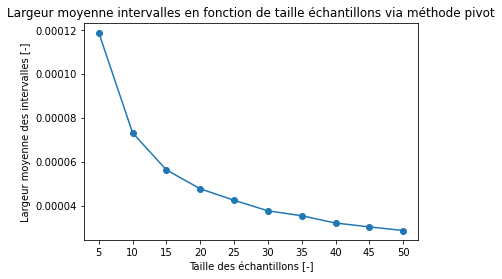
\includegraphics[width=8cm]{pivot.png}
        \caption{}
        \label{Débit_frottement}
    \end{minipage}
    \hspace{0.55cm}
    \begin{minipage}{.5\textwidth}
        \centering
        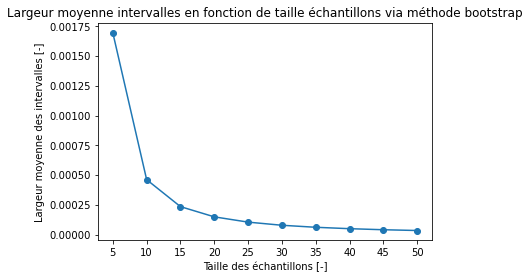
\includegraphics[width=8cm]{bootstrap.png}
        \caption{}
        \label{Pression_frottement}
    \end{minipage}
\end{figure}\\\\
Ces deux graphiques mettent en exergue que les intervalles de confiance fournis par la méthode du pivot ont une largeur moyenne plus faible que les intervalles de confiance fournis par la méthode du bootstrap. Cependant, on remarque également que les deux graphiques présentent une similitude : une forte décroissance exponentielle qui fini par converger.
    \item Ensuite, sur base des mêmes échantillons qu'au point (e) (de 5 à 50 par pas de 5), nous analysons la proprotion d'intervalles parmi les 500 qui contiennent le véritable $\lambda$, celui-ci étant $\lambda=5,247\times10^{-5}$. La figure ci-dessous représente l'évolution de cette propotion en fonction de la taille des échantillons pour les deux méthodes :
        \begin{figure}[h!]
    \begin{minipage}{.5\textwidth}
        \centering
        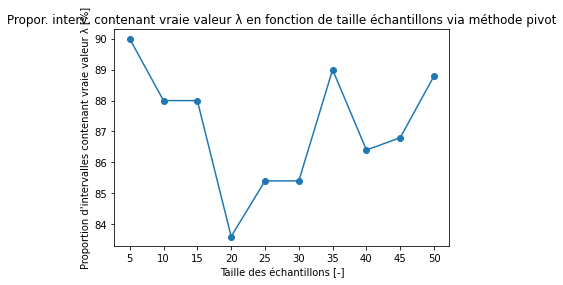
\includegraphics[width=8cm]{proportion_pivot.png}
        \caption{}
        \label{Débit_frottement}
    \end{minipage}
    \hspace{0.55cm}
    \begin{minipage}{.5\textwidth}
        \centering
        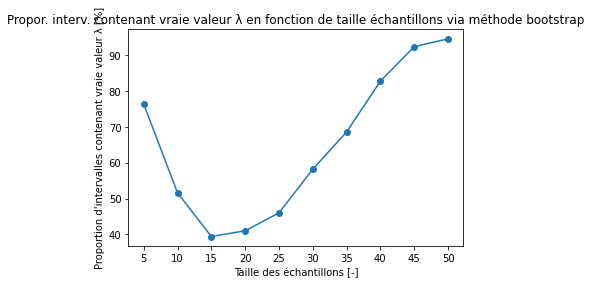
\includegraphics[width=8cm]{proportion_bootstrap.png}
        \caption{}
        \label{Pression_frottement}
    \end{minipage}
\end{figure}\\\\
En voyant ces deux graphiques, on remarque que l'évolution de la proportion d'intervalles contentenant le vrai $\lambda$ en fonction de la taille des échantillons pour la méthode du pivot n'est pas du tout fluide alors que l'évolution pour la méthode du bootstrap l'est. Cependant, on remarque également que la méthode du pivot à une moyenne de proportion d'intervalles contenant le vrai $\lambda$ beaucoup plus élevée que la méthode du bootstrap. En effet, cette proportion ne descend pas en dessous de $83\%$ pour la méthode du pivot, alors qu'elle est parfois inférieure à $40\%$ pour la méthode du bootstrap.
 \item A la lumière de l'ensemble de ces résultats, il apparaît qu'il était pertinent de supposer que l'échantillon de $PIB\_habitant$ suivait une distribution exponentielle. En effet, on remarque que les intervalles de confiance sont assez réduits et que la proportion d'intervalle contenant  le vrai $\lambda$ est assez élevée, ce qui signifie que cet échantillon se rapproche correctement d'une distribution exponentielle.
\end{enumerate}

\section{Test d'hypothèse}
\begin{enumerate}[label=(\alph*)]
    \item Dans cette section, nous réalisons un test d'hypothèse. On souhaite savoir si la moyenne d'émission de $CO_2$ des pays riches est égale à la moyenne des émission de $CO_2$ des pays pauvres plus un certain $\Delta$ (déterminé à l'aide de la fonction $\textbf{scientific\_delta}$) ou si la différence est supérieure à ce $\Delta$. Pour ce faire, on émet les deux hypothèses suivantes :
\begin{center}
    $H_0$ : La différence d'émission de $CO_2$ vaut $\Delta$\\
    $H_1$ : La différence d'émission de $CO_2$ est supérieure à $\Delta$
\end{center}\\
Sachant qu'un pays est considéré comme riche si son $PIB/Habitants$ est supérieur au $PIB/Habitants$ médian, et qu'il est considéré comme pauvre le cas échéant, nous pouvons chercher quelle hypothèse est vraie dans notre population. En utilisant la fonction citée plus tôt, on remarque aisément que c'est $H_0$ qui se réalise, et donc que la différence des émissions des $CO_2$ des pays riches et pauvres est belle et bien égale à la valeur fournie par $\textbf{scientific\_delta}$.
\item Ensuite, on souhaite réaliser un test d'hypothèse au seuil de signification $\alpha=5\%$, en d'autres termes, tel que la probabilité que $H_0$ soit rejeté est inférieure à 0,05. Pour ce faire, nous déterminons une zone de rejet sur la variable d'intérêt, c'est-à-dire une zone où la probabilité que la variable s'y trouve, et donc soit rejetée, est inférieure à $0,05$. D'une manière plus concrète, soit la variable aléatoire $X$ représentant l'émission de $CO_2$ d'un pays riche et la variable aléatoire Y représentant l'émission de $CO_2$ d'un pays pauvre. Si l'on suppose que les échantillons sont de taille relativement grande, on peut y appliquer le théorème central limite. Les deux variables aléatoires ayant par hypothèse la même variance, appelée $\sigma$, il vient:
\begin{center}
    $X\sim\mathcal{N}(m_r,\sigma^2/n_r)$ et $Y\sim\mathcal{N}(m_p,\sigma^2/n_p)$
\end{center}
Ce test d'hypothèse repose sur la différence entre ces deux variables. Par conséquent, soit $Z$ étant la variable aléatoire sur laquelle nous construirons notre zone de rejet :
$$Z=\overline{X}-\overline{Y}$$
En utilisant les propriétés de la loi normale, nous pouvons aisément déterminer la distribution de cette variable. Il vient:
$$Z\sim\mathcal{N}(m_r-m_p,\sigma^2\left(\frac{1}{n_r}+\frac{1}{n_p}\right))$$
Le test d'hypothèse que nous réalisons prend dès lors la forme:
\begin{center}
    $H_0~:~m_r-m_p=\Delta$ et $H_1~:~m_r-m_p>\Delta$
\end{center}
Puisque la moyenne et la variance de la variable $Z$ sont inconnues, nous utilons une loi normale centrée réduite. Nous avons dès lors:
$$T=\frac{Z-(m_r-m_p)}{\sigma\sqrt{\left(\frac{1}{n_r}+\frac{1}{n_p}\right)}}\sim\mathcal{N}(0,1)$$
Puisque nous ne connaissons pas la variance $\sigma$, nous allons chercher à l'estimer grâce à la variable $S$. Soit $S^2_x$ une estimation de la variance de $X$ et $S^2_y$ une estimation de la variance de $Y$. Il vient :
\begin{center}
$S^2_x=\frac{1}{n_r-1}\sum_{i=1}^{n_r} (X_i-\overline{X})^2$ et $S^2_y=\frac{1}{n_p-1}\sum_{i=1}^{n_p} (Y_i-\overline{Y})^2$
\end{center}
\newpage
En suivant la théorie de la distribution normale nous savons que si :
\begin{center}
    $\frac{(n_r-1)S_x^2}{\sigma^2}\sim \chi_{(n_r-1)}^2$, et ce indépendament de $\frac{(n_p-1)S_y^2}{\sigma^2}\sim \chi_{(n_p-1)}^2$
\end{center}
Il vient alors :
$$(n_r-1)\frac{S^2_x}{\sigma^2}+ (n_p-1)\frac{S_y^2}{\sigma^2}\sim \chi^2_{n_r+n_m-2}$$
Par conséquent, nous pouvons estimer la valeur de $S$ en mettant en commun les estimations séparées de $X$ et $Y$. On a :
$$S^2=\frac{1}{n_r+n_p-2}\left(\sum^{n_r}_{i=1}(X_i-\overline{X})^2+\sum^{n_p}_{i=1}(Y_i-\overline{Y})^2\right)= \frac{(n_r-1)S^2_x+(n_p-1)S^2_y}{n_r+n_p-2}$$
Dès lors, nous connaissons la valeur de $S$ dans un cas précis, mais dans cet exposé théorique, nous nous intéressons à sa distribution. Nous savons que :
$$S\sim\chi^2_{n_r+n_m-2}$$
En conséquence la distribution de $T$ devient :
$$T\sim\frac{\mathcal{N}(0,1)}{\chi^2_{n_r+n_p-2}}=t_{n_r+n_p-2}$$
Nous souhaitions un test d'hypothèse au seuil de signification de $5\%$. En d'autre termes, cela signifie que la probabilité que l'hypothèse $H_0$ soit réalisée doit être supérieure à $100\%-5\%=95\%$. Si l'on se place dans le cas de l'hypothèse $H_0$, qui a une probabilité de 0,95 de se produire, nous obtenons notre zone de rejet, donnée par:
$$\frac{Z-\Delta}{S\sqrt{\left(\frac{1}{n_r}+\frac{1}{n_p}\right)}}>t_{n_r+n_p-2;0,95}$$
Par conséquent, les valeurs de $Z$ qui satisfont ces conditions provoquent une réalisation de $H_1$, et ce avec un probabilité inférieure à 0,05.
\item Nous allons mettre les résultats obtenus au point précédent en aplication. Pour ce faire, nous tirons 100 échantillons de 75 pays dans notre population de 150 pays. Sur chacun des échantillons, nous allons tester l'hypothèse au seuil de signification $\alpha=5\%$. Parmi ces échantillons, l'hypothèse nulle $H_0$ est rejetée à seulement 2 reprises. Ce résultat est bon puisque nous voulions une probabilité de rejet inférieure à 0,05, mais pas parfait. En effet, théoriquement, la probabilité de rejet de l'hypothèse $H_0$ attendue est 0,05. Dès lors, puisque nous réalisons 100 tirages, nous aurions du avoir 5 rejets de l'hypothèse. Cet éloignement est dû au fait que cette zone de rejet se base sur une distribution théorique, et non pas sur la distribution empirique, qui diffère légèrement.
\item Ensuite, nous répétons la même opération avec, cette fois, 100 échantillons de 25 pays. Dans ce cas ci, l'hypothèse nulle $H_0$ est rejetée à 5 reprises. Ce qui correspond au résultat théorique attendu. Cela est dû au fait que nous prenons des échantillons de seulement 25 pays et, comme vu au point 2 de ce rapport, les estimations sont moins qualitatives, et par conséquent, l'hypothèse est rejetée davantage de fois.
\end{enumerate}
\end{document}
